\chapter{Cosmological Surveys}
There are many projects and missions which study properties of the dark energy, either as a main scientific goal, or as a complementary program. Among the big surveys are e.g. Sloan Digital Sky Surveys (SDSS, \cite{SDSS}) which aims to create the most detailed three-dimensional maps of the Universe. From the beginning of regular surveys in 2000 till 2014 there were seven finished surveys in total (SDSS-I/II results \cite{SDSS_I_II}, SDSS-III results \cite{BOSS_results}), while there are three ongoing surveys from 2014 (SDSS-IV, \cite{2017AJ....154...28B}) and a planned panoptic spectroscopic survey (SDSS-V, \cite{2017arXiv171103234K}) which will start collecting data in summer 2020. Other surveys are e.g. Wilkinson Microwave Anisotropy Probe (WMAP, \cite{WMAP}, results \cite{WMAP_results}); Planck (\cite{planck}, results \cite{planck_cosm}). There are also several planned surveys almost ready to start collecting data -- Euclid \parencite{euclid}, LSST \parencite{lsst} or W-FIRST \parencite{WFIRST_report}.

\section{BOSS}
The Sloan Digital Sky Survey`s (SDSS-III) Baryon Oscillation Spectroscopic Survey (BOSS) is a six-year program (Fall 2009 -- Spring 2014)  that uses the wide-field 2.5-m telescope at Apache Point Observatory, see \autoref{fig:sdss_tele}. The BOSS is designed to measure the scale of BAO in the clustering of matter over a larger volume than the combined efforts of all previous spectroscopic surveys of large-scale structures. BOSS uses 1.5 million luminous galaxies to measure BAO to redshifts $z<0.7$. Observations of neutral hydrogen in the Ly$\alpha$ forest in more than 150,000 quasar spectra constrain BAO over the redshift range $2.15 < z < 3.5$ \cite{BOSS}.
\begin{figure}[ht]
    \centering
    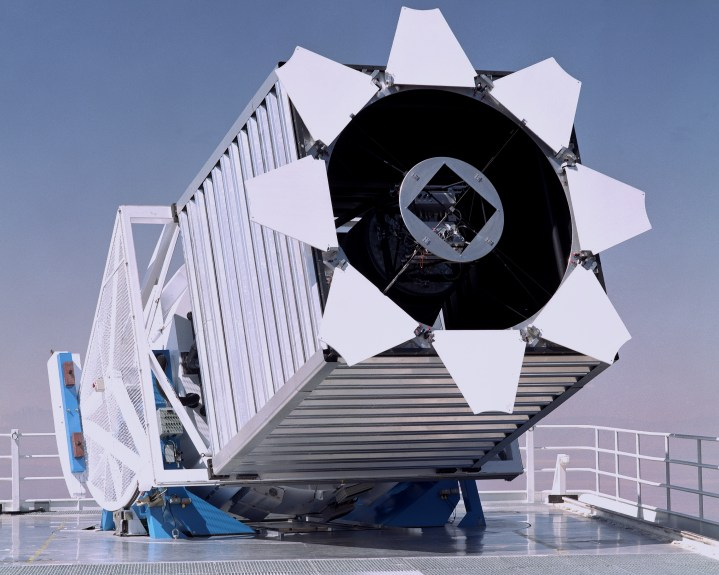
\includegraphics[width=\textwidth]{cosmo_surveys/SDSS_telescope_new.jpg}
    \caption{Sloan Foundation 2.5m Telescope.}
    \label{fig:sdss_tele}
\end{figure}

There are two double spectrographs, each covering the wavelength range 361 nm -- 1014 nm with resolution $R=\lambda/\Delta\lambda$ ranging from 1300 at the blue end to 2600 at the red end.  Both spectrographs have a red channel with a 4k $\times$ 4k, 15\um  pixel CCD from Lawrence Berkeley National Laboratory (LBNL). Both spectrographs have a blue channel with a 4k $\times$ 4k, 15\um  pixel CCD from  e2v. The instrument is fed by 1000 optical fibers (500 per spectrograph), each subtending 2'' on the sky.

Using the acoustic scale as a physically calibrated ruler, BOSS determines the angular diameter distance with a precision of 1\% at redshifts $z = 0.3$ and $z = 0.57$ using the distribution of galaxies and measurements of $H(z)$ to 1.8\% and 1.7\%  at the same redshifts. At redshifts $z\sim2.5$ the  angular diameter distance and $H\mins(z)$ is measured to an accuracy of 1.9\% using Ly$\alpha$ forest.

BAO measurements with the CMB-calibrated physical scale of the sound horizon and SN data yields of $H_0=(67.3\pm1.1)$ \unith\ with 1.7\% precision \cite{BOSS_results}. This measurement assumes standard pre-recombination physics but is insensitive to assumptions about dark energy or space curvature. When we allow more general forms of evolving dark energy, the BAO+SN+CMB parameter constraints are always consistent with flat \LCDM\ values at $1\sigma$. While the overal $\chi^2$ of model fits is satisfactory, the Ly$\alpha$ forest BAO measurements are in moderate $(2-2.5\sigma)$ tension with model predictions. Models with early dark energy that tracks the dominant energy component at high redshift remain consistent with expansion history constraints, and they yield a higher $H_0$ and lower matter clustering amplitude, improving agreement with some low-redshift observations.

\section{eBOSS}
The Extended Baryon Oscillation Spectroscopic Survey (eBOSS, \cite{2016AJ....151...44D}) is the new cosmological survey within a SDSS-IV six-year program started in 2014 July. eBOSS will conduct novel cosmological observations of galaxies, and in particular quasars, using the same 1000-fiber optical spectrographs as those in BOSS at Apache Point Observatory. These observations will be conducted simultaneously with the Time Domain Spectroscopic Survey (TDSS, \cite{2015ApJ...806..244M}) designed for variability studies and the Spectroscopic Identification of eROSITA Sources (SPIDERS, \cite{2010SPIE.7741E..1NF}) program designed for studies of X-ray sources.

eBOSS will map the large-scale-structures over the relatively unconstrained redshift range $0.6<z< 2.2$, see \autoref{fig:eboss} for comparison with BOSS range. eBOSS will expand the selection of luminous red galaxies (LRG) beyond that probed by BOSS and obtain better than a $1.0\%$ precision distance estimate when combined with the $z > 0.6$ tail of the BOSS galaxy population. With observations of a new sample of emission line galaxies (ELG) eBOSS will produce a $2.0\%$ precision distance estimate at higher redshifts. eBOSS will obtain a $1.8\%$ precision distance estimate in the redshift range $0.9 < z < 2.2$ using quasars that have luminosities and areal densities well-suited to sensitivity of the BOSS spectrographs. Finally, eBOSS will sharpen the BOSS Ly$\alpha$ forest measurements by a factor of $1.44$ with a new selection of $z > 2.1$ quasars, providing stronger leverage on the history of dark energy.
\begin{figure}[ht]
    \centering
    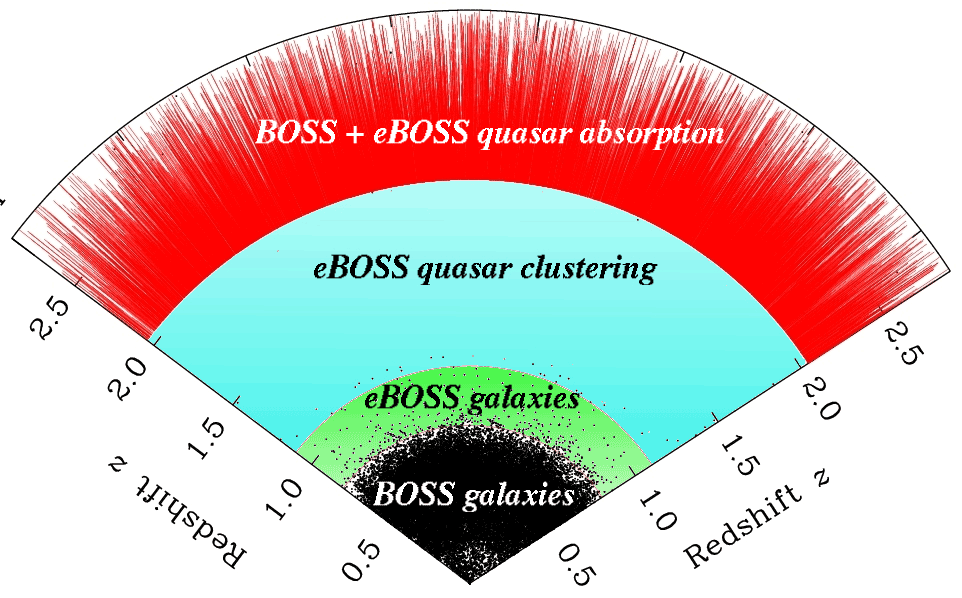
\includegraphics[width=\textwidth]{cosmo_surveys/pie_boss_eboss_marked.png}
    \caption{Planned eBOSS coverage of the Universe.}
    \label{fig:eboss}
\end{figure}

With four classes of spectroscopic targets (LRG, ELG, quasar, Ly$\alpha$ forest quasar), eBOSS will enable the first high precision distance measurements in the epochs when dark energy emerged as the dominant dynamical component of the Universe. In addition to BAO distance measurements, eBOSS will provide new tests of GR on cosmological scales through redshift-space distortions (RSD), new tests for non-Gaussianity in the primordial density field, and new constraints on the summed mass of all neutrino species.


\section{DES}
\label{DES}
The Dark Energy Survey (DES) is designed to probe the origin of the accelerating universe and to help uncover the nature of dark energy by measuring the \mbox{14-billion-year} history of cosmic expansion with high precision. DES is an optical near infrared survey of 5000 deg\sq\ of the South Galactic Cap to $r\sim24$ in $grizy$ spectrum. DES`s instrument consists primarily of a new camera, Dark Energy Camera (DECam), specifically designed to be sensitive to the highly redshifted light from distant galaxies. DECam is mounted on a classic telescope, the Blanco 4-m telescope at the Cerro Tololo Inter-American Observatory (CTIO) in La Serena, Chile. The imaging system is supported by a combination of microwave and optical data links that will provide the recorded data to the survey members. Starting in August of 2013 and continuing for five years, DES has begun to survey a large swath of the southern sky out to vast distances in order to provide new clues to this most fundamental questions \cite{DES}.

\begin{figure}[ht]
    \centering
    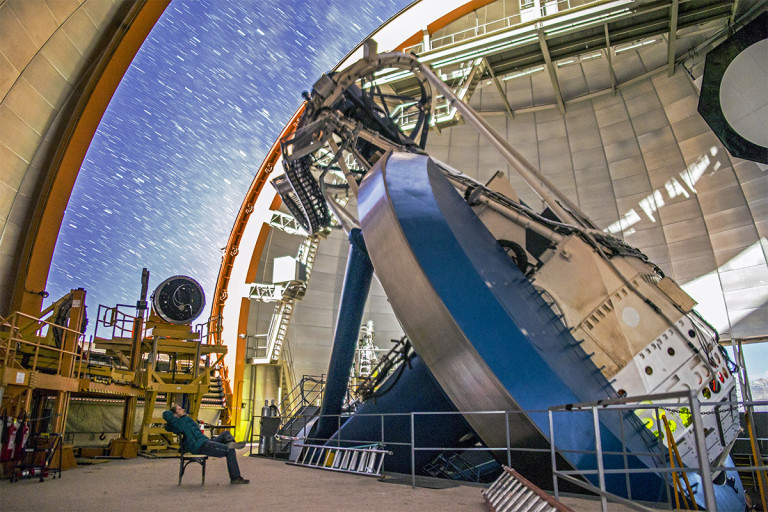
\includegraphics[width=\textwidth]{cosmo_surveys/des.jpg}
    \caption{DESCam operating at night, while an observer watches.}
    \label{fig:des}
\end{figure}
The survey data allow to measure the dark energy and dark matter densities and the dark energy equation of state through four independent methods: galaxy clusters (counts and spatial distributions at $0.1<z<1.3$), weak gravitational lensing tomography (on several redshift shells to $z\sim1$), galaxy angular clustering, and supernova distances (at $0.3<z<0.8$).

The main tool is the DECam, 74 2k $\times$ 4k 570 Mpx digital camera built at Fermilab in Batavia. It provides a 2.2\textdegree field of view image at 0.27''/pixel. It covers wavelength range 400--1100 nm with five filters $(grizy)$. The electronics will allow an entire digital image to be read out and recorded in 17 seconds, time that it takes the telescope to move to its next viewing position.

From the first two years of observation a mass map from weak gravitational lensing shear measurements over 139 deg\sq\ has been reconstructed \cite{DES_mass}. There is a good agreement between the mass map and the distribution of massive galaxy clusters identified using a red-sequence cluster finder. These measurements are consistent with simulated galaxy catalogs based on \LCDM\ \nbody s, suggesting low systematics uncertainties in the map.


\section{Euclid}
Euclid is an ESA (European Space Agency) high-precision space mission in ESA`s Cosmic Vision 2015--2025 scientific programme designed to map the geometry and evolution of the universe and to study properties of dark matter and dark energy. Its primary goal is to place high accuracy constraints on dark energy, dark matter, gravity and cosmic initial conditions using two independent cosmological probes -- weak gravitational lensing and baryonic acoustic oscillation -- out to redshift $z\sim2$. Galaxy clusters and the Integrated SachsWolfe effect will be used as secondary cosmological probes. Along with these tasks will Euclid`s visible and near infrared imaging and spectroscopy of the entire extragalactic sky produce legacy science for various fields of astronomy, e.g. galaxy evolution, large-scale structures or the search for high-redshift objects. The Euclid mission has been adopted with the mission`s timeframe for liftoff starting in mid-2022 from the Guiana Space Centre, Europe`s Spaceport in French Guiana. Overview of the Euclid system design and scientific requirements can be found in \cite{2011arXiv1110.3193L}.

\begin{figure}[ht]
    \centering
    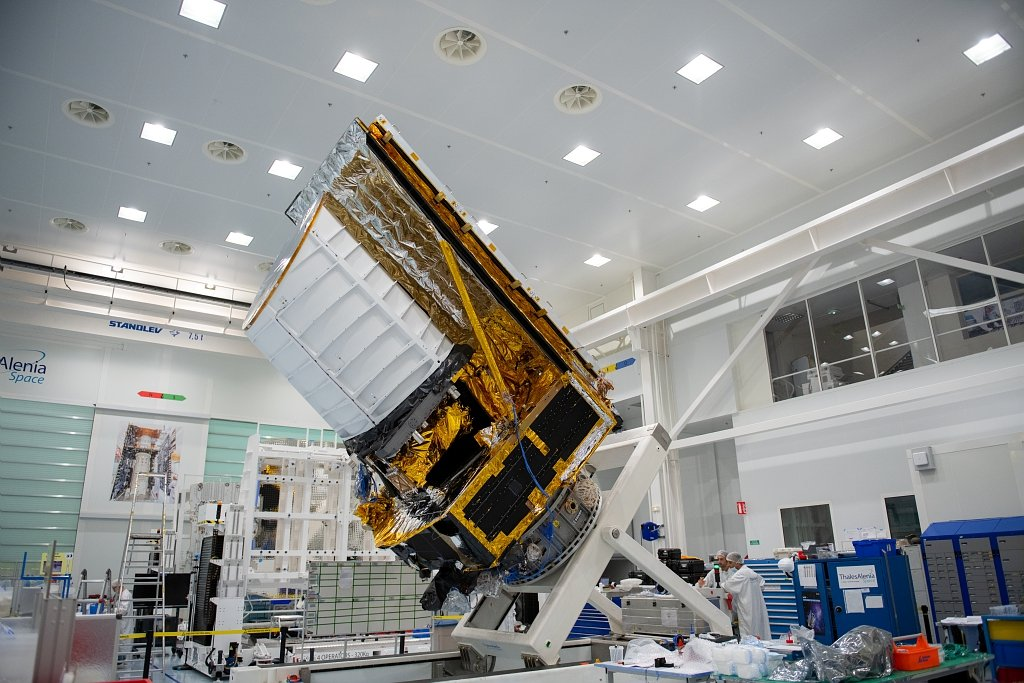
\includegraphics[width=\textwidth]{cosmo_surveys/euclid.jpg}
    \caption{Structural and thermal model of the Euclid satellite.}
    \label{fig:euclid}
\end{figure}
\subsection{The Euclid Consortium}
The Euclid Consortium (EC) is an organisation that brings together teams of researchers in theoretical physics, particle physics, astrophysics and space astronomy, and also engineers, technicians, and management and administrative staffs working in public research laboratories and contributing to the Euclid mission. Together with the European Space Agency (ESA) and aerospace industry they are part of the Euclid Collaboration. The EC has been selected by ESA in June 2012 as the single official scientific consortium having the responsibility of the scientific instruments, the production of the data and of leading the scientific exploitation of the mission until completion. It is funded by national space agencies and national research organizations and led by the Euclid Consortium Lead (ECL) and a Euclid Consortium Board (ECB). The ECL and ECB are the primary contact points with ESA and with the Euclid Consortium members.

\section{Large Synoptic Survey Telescope}
The Large Synoptic Survey Telescope (LSST, \cite{lsst}) is a ground-based telescope being built in northern Chile on the Cerro Pach\'{o}n mountain. The system will produce a 6-band (300 -- 1100 nm) wide-field deep astronomical survey over 20,000 deg\sq\ of the southern sky. Combining the wide field of view with short exposures, the LSST will take more than 800 images each night and cover the whole observable sky twice each week. Each patch of the sky will be visited about 1000 times during ten years. The LSST will provide an unprecedented depth (single-visit 24.5 mag, co-added 27.5 mag) and unique details of the Universe while producing 30 terabytes of data nightly. This data will be used for locating dark matter and to characterize the properties of the dark energy. Other major tasks for the LSST will be detecting and tracking potentially hazardous asteroids or studying the structure of the Milky Way. The project is in the construction phase and will begin regular survey operations by 2022.

\subsection{Vera C. Rubin Observatory}
\begin{figure}[ht]
    \centering
    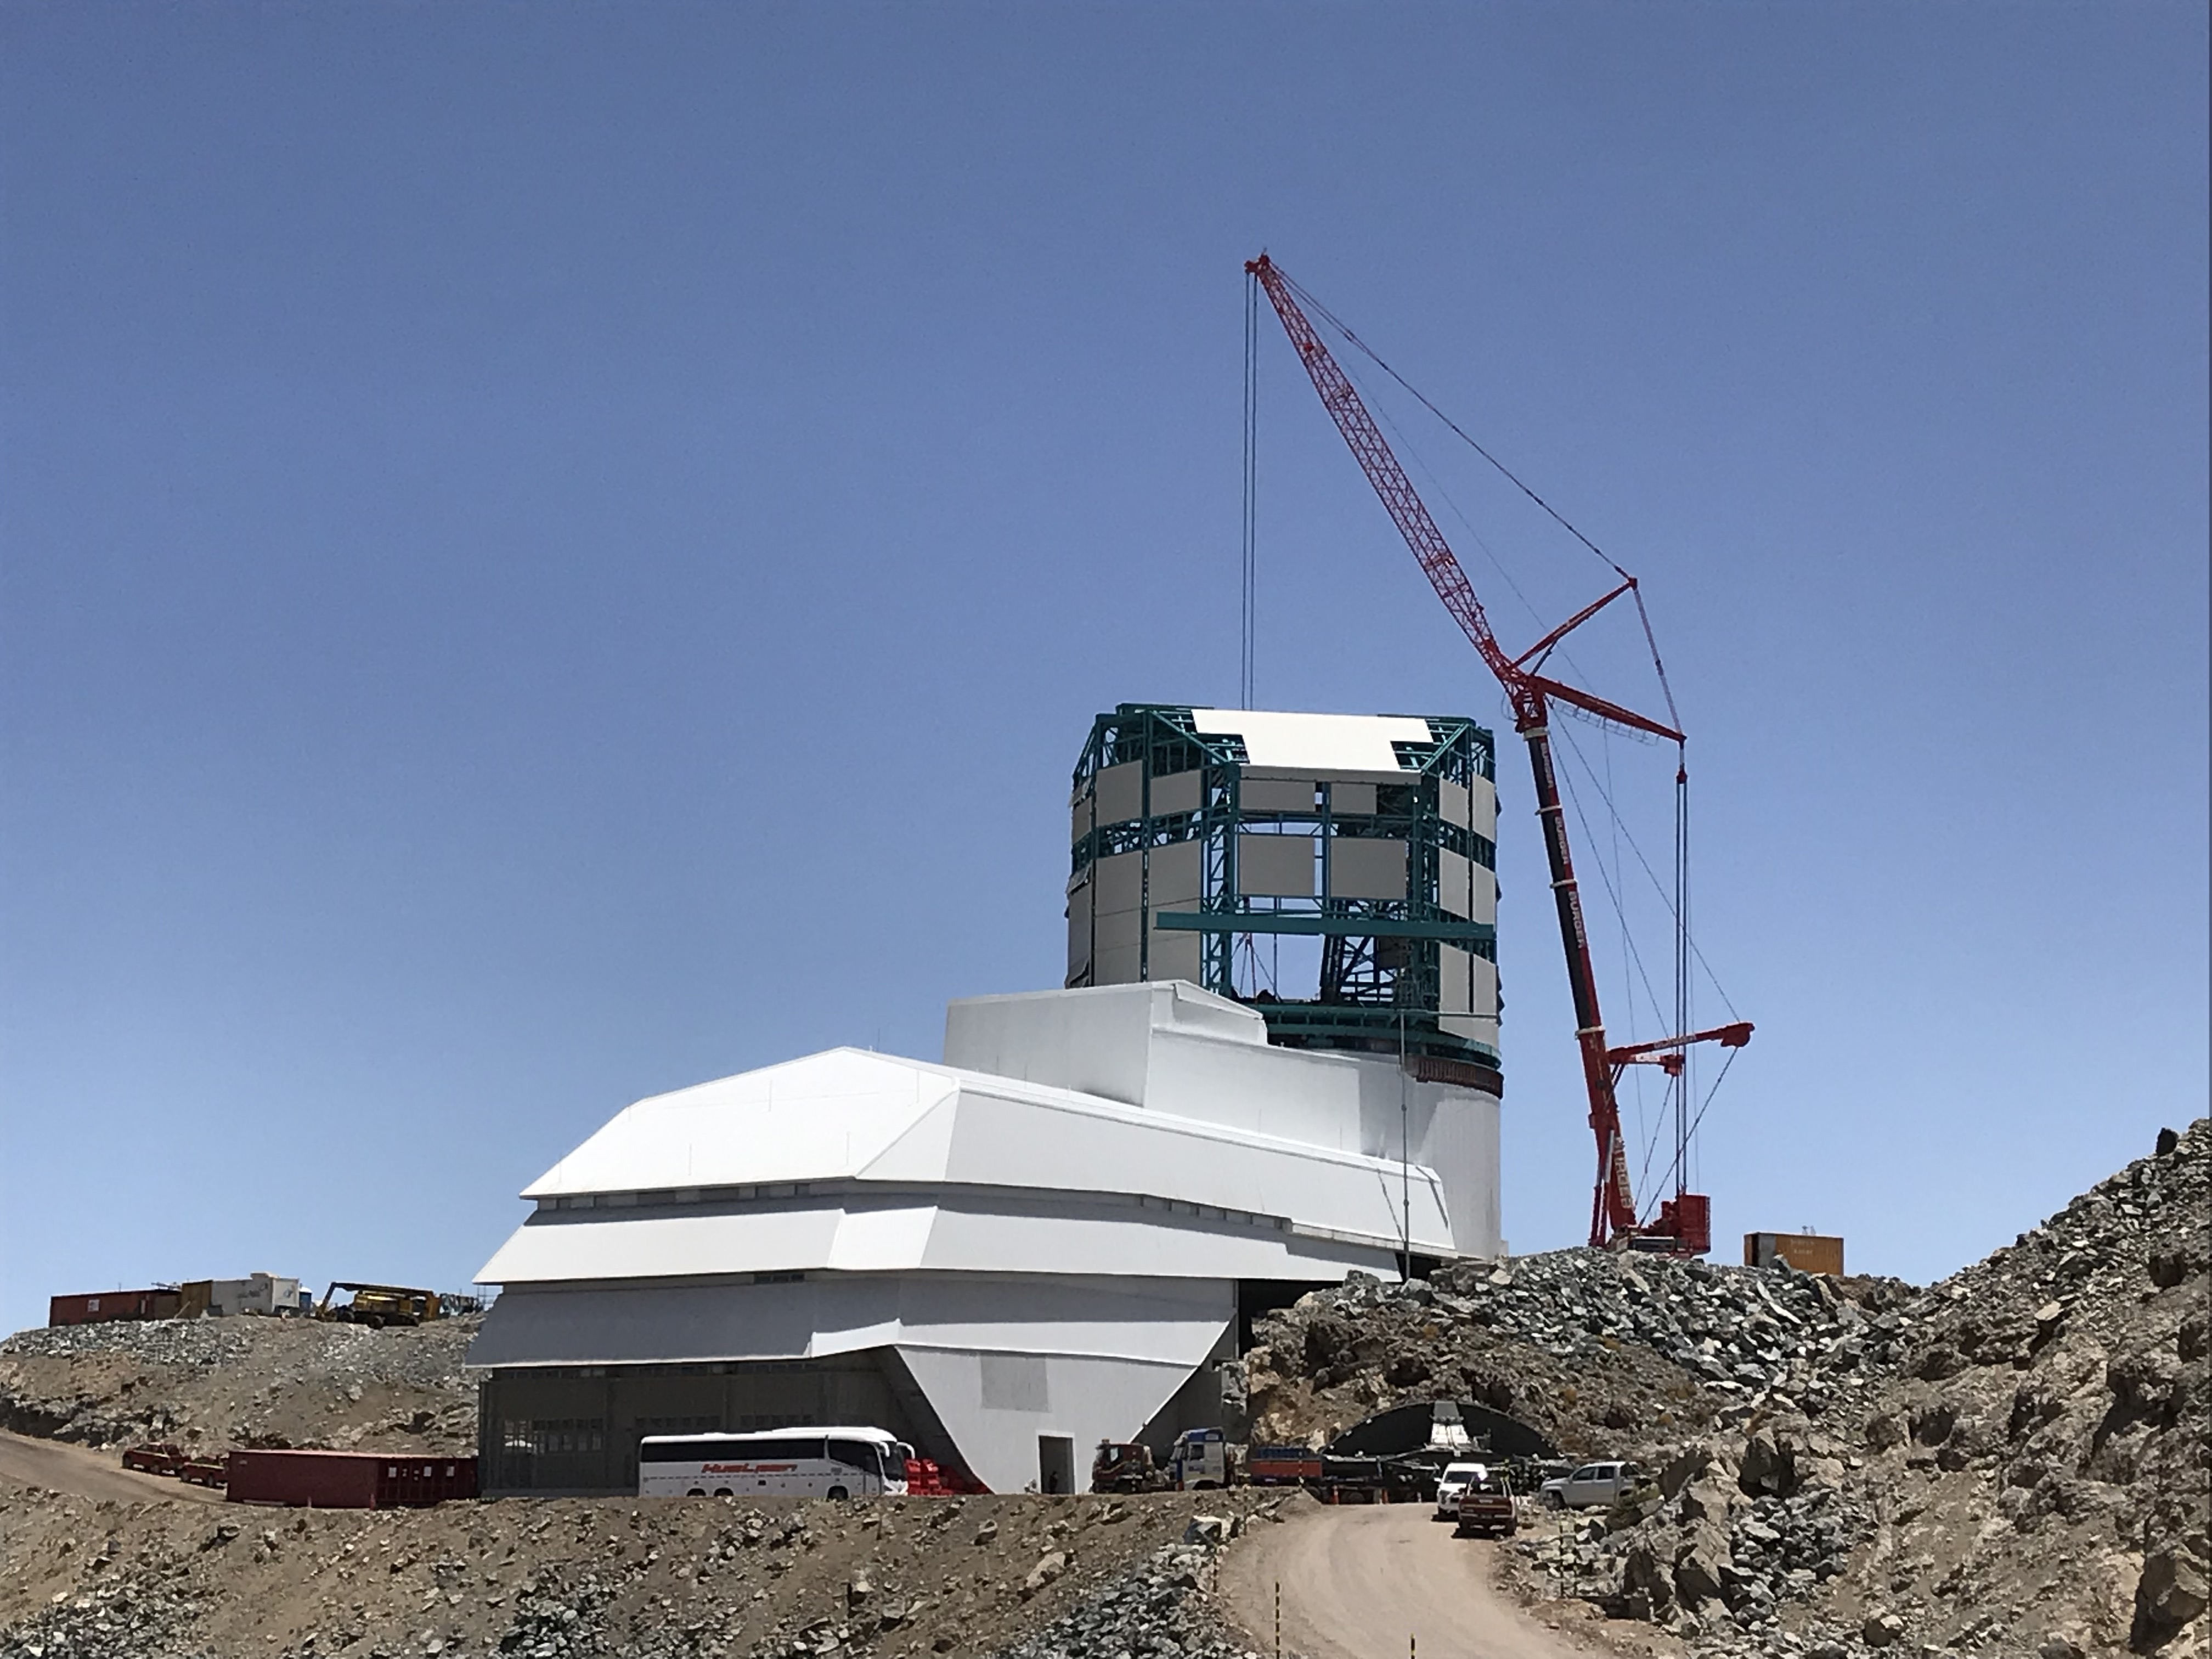
\includegraphics[width=\textwidth]{cosmo_surveys/lsst_site.jpg}
    \caption{Construction on the Vera C. Rubin Observatory. Most of the large pieces of equipment have arrived on the summit, and installation of the Telescope Mount Assembly (TMA) began in early 2020. Credit: LSST Project/NSF/AURA}
    \label{fig:lsst_site}
\end{figure}
On Januray 6, 2020, it was announced that the LSST will be named the NSF (National Science Foundation) Vera C. Rubin Observatory (Rubin Observatory) after an astronomer who provided important evidence of the existence of dark matter. Rubin Observatory Director Steve Kahn said,

\textit{``We are deeply honored to have our observatory named after Vera Rubin, who is most well known for her work measuring the discrepancy between observed rotational motions of galaxies and their predicted motion, which provided strong evidence for the existence of dark matter. Vera made one of the most important contributions to science in the past century, not only for astronomy, but also for fundamental physics. When construction is completed in 2022, the Rubin Observatory and the LSST Camera will help build on her pioneering work to dramatically improve our understanding of the Universe on many different scales.''}

NSF also announced on Januray 6, 2020, that the telescope at the Rubin Observatory will be named the Simonyi Survey Telescope in recognition of the significant private donation made through the Corporation early in the construction phase in support of the design, development, and fabrication of the telescope`s primary mirror. 

\subsection{Observatory Site}
The LSST will be constructed on Cerro Pach\'{o}n in the northern Chilean Andes. This site was chosen after an extensive study comparing seeing conditions, cloud cover and other weather patterns. The expected mean delivered image quality is $0.67''$ in $g$-band as measured by differential image motion monitoring (DIMM) on Cerro Tololo. The excellent image quality have been confirmed also by nearby 8.2-m diameter Gemini-South and 4.3-m diameter Southern Astrophysical Research (SOAR) telescopes.

The LSST Observatory as a whole will be distributed over four sites: the Summit Facility on El Pe$\tilde{\mbox n}$\'{o}n, the Base Facility, the Archive Center, and the Data Centers. The Base Facility will be at the AURA compound in the town of La Serena, 57 km away from the mountain. The Archive Center will be at the National Center for Supercomputing Applications (NCSA) on the campus of the University of Illinois at Urbana-Champaign. One of the two Data Centers will be located with the Archive Center at NCSA and the other one at the Base Facility in La Serena. All these facilities will be connected via dedicated high-bandwidth fiber optic links.

The exterior of the summit facility building is nearly complete, see \autoref{fig:lsst_site}. Inside, major components of the telescope have begun to arrive from their places of manufacture around the globe, including the mirror washing and coating equipment, and the Secondary Mirror (M2) and its support system.
\subsection{Telescope}
The LSST telescope consists of three aspheric mirrors -- an 8.4-m primary M1, a 3.4-m convex secondary M2 (the largest convex mirror ever made), and a 5.0-m tertiary M3. The primary mirror is highly annular having an outer clear aperture of 8.36 m and an inner diameter of 5.12 m, giving an effective collecting area of a 6.67-m filled aperture. The camera body and its associated readout electronics are located in the 1.8-m diameter hole in the secondary mirror.  The hole in the tertiary mirror is used to mount equipment for the maintenance of the LSST optical alignment. The primary and tertiary mirrors form a continuous surface without any vertical discontinuities.

The M1-M3 monolith (see \autoref{fig:lsst_m1m3}) was completely formed and polished in February 2015 after seven years of casting at Steward Observatory Mirror Lab at the University of Arizona. On May 19th 2015, the completed LSST Primary/Tertiary mirror (M1M3) was safely moved from the UA's Richard F. Carris Mirror Lab (formerly SOML) to long-term secure storage at Tucson International Airport. In late 2018 the mirror was returned to the Mirror Lab for optical testing, and in early 2019 it was shipped to the summit facility on Cerro Pach\'{o}n. The secondary mirror is made of a low expansion glas using a 100 mm-thick solid meniscus blank. The mirror is supported above and facing the M1M3 monolith and the alignment of the three mirror surfaces is maintained using systems of actuators -- small motors that can make tiny adjustments to the position of the mirror from several angles. A large conical baffle prevents the direct reflection of starlight from the tertiary mirror into the camera.
\begin{figure}[ht]
    \centering
    \includegraphics[width=\textwidth]{cosmo_surveys/lsst_m1m3.jpg}
    \caption{The LSST Primary/Tertiary Mirror (M1M3) in the Richard F Caris Mirror Lab at the University of Arizona for optical testing. In May, 2019, the mirror reached its new home in the Andes Mountains of Northern Chile. Credit: LSST Project/NSF/AURA}
    \label{fig:lsst_m1m3}
\end{figure}

The proposed LSST telescope (see \autoref{fig:lsst_tma}) is a compact, stiff structure with a powerful set of drives, which makes it very accurate and agile. The telescope structure is a welded and bolted steel system designed to be a stiff metering structure for the optics and a stable platform for observing. The primary and tertiary mirrors are supported in a single cell below the elevation ring, the camera and secondary mirror are supported above it. This construction makes it possible to reorient the telescope very quickly -- the motion time for a nominal 3.5\textdegree elevation move and a 7\textdegree azimuth move is only five seconds. In two seconds, a shaped control profile will move the telescope, which will then settle down to less than $0.1"$ pointing error in three seconds. There are four motors per axis configured in two sets of opposing pairs to eliminate hysteresis in the system. All-sky pointing performance will be better than $2"$, which is important for trailing and imaging systematics.
\begin{figure}[ht]
    \centering
    \includegraphics[width=\textwidth]{cosmo_surveys/lsst_tma.jpg}
    \caption{The construction of the LSST Telescope Mount Assembly (TMA) was a concerted effort by many people. This group photo was taken just before disassembly work began on the TMA in preparation for shipping it to Chile.. Credit: Asturfeito}
    \label{fig:lsst_tma}
\end{figure}

\subsection{Camera}
The LSST camera (see \autoref{fig:lsst_cam_des}) with size of 1.6 meters by 3 meters and weight of 2800 kilograms will be the largest digital camera ever constructed. It will produce data of extremely high quality with minimal downtime and maintenance. It is a large-aperture, wide-field optical (0.3--1 \um) imager designed to provide a 3.5\textdegree field of view with sampling better than 0.2 arcsecond. The image surface is flat with a diameter of approximately 64 cm. Used detectors are 16 Mpixel silicon detectors providing a total of approximately 3.2 Gpixels with read out in 2 sec (15 sec integration). The camera has 6 filters ($ugrizy$) and is located in the middle of the telescope.
\begin{figure}[ht]
    \centering
    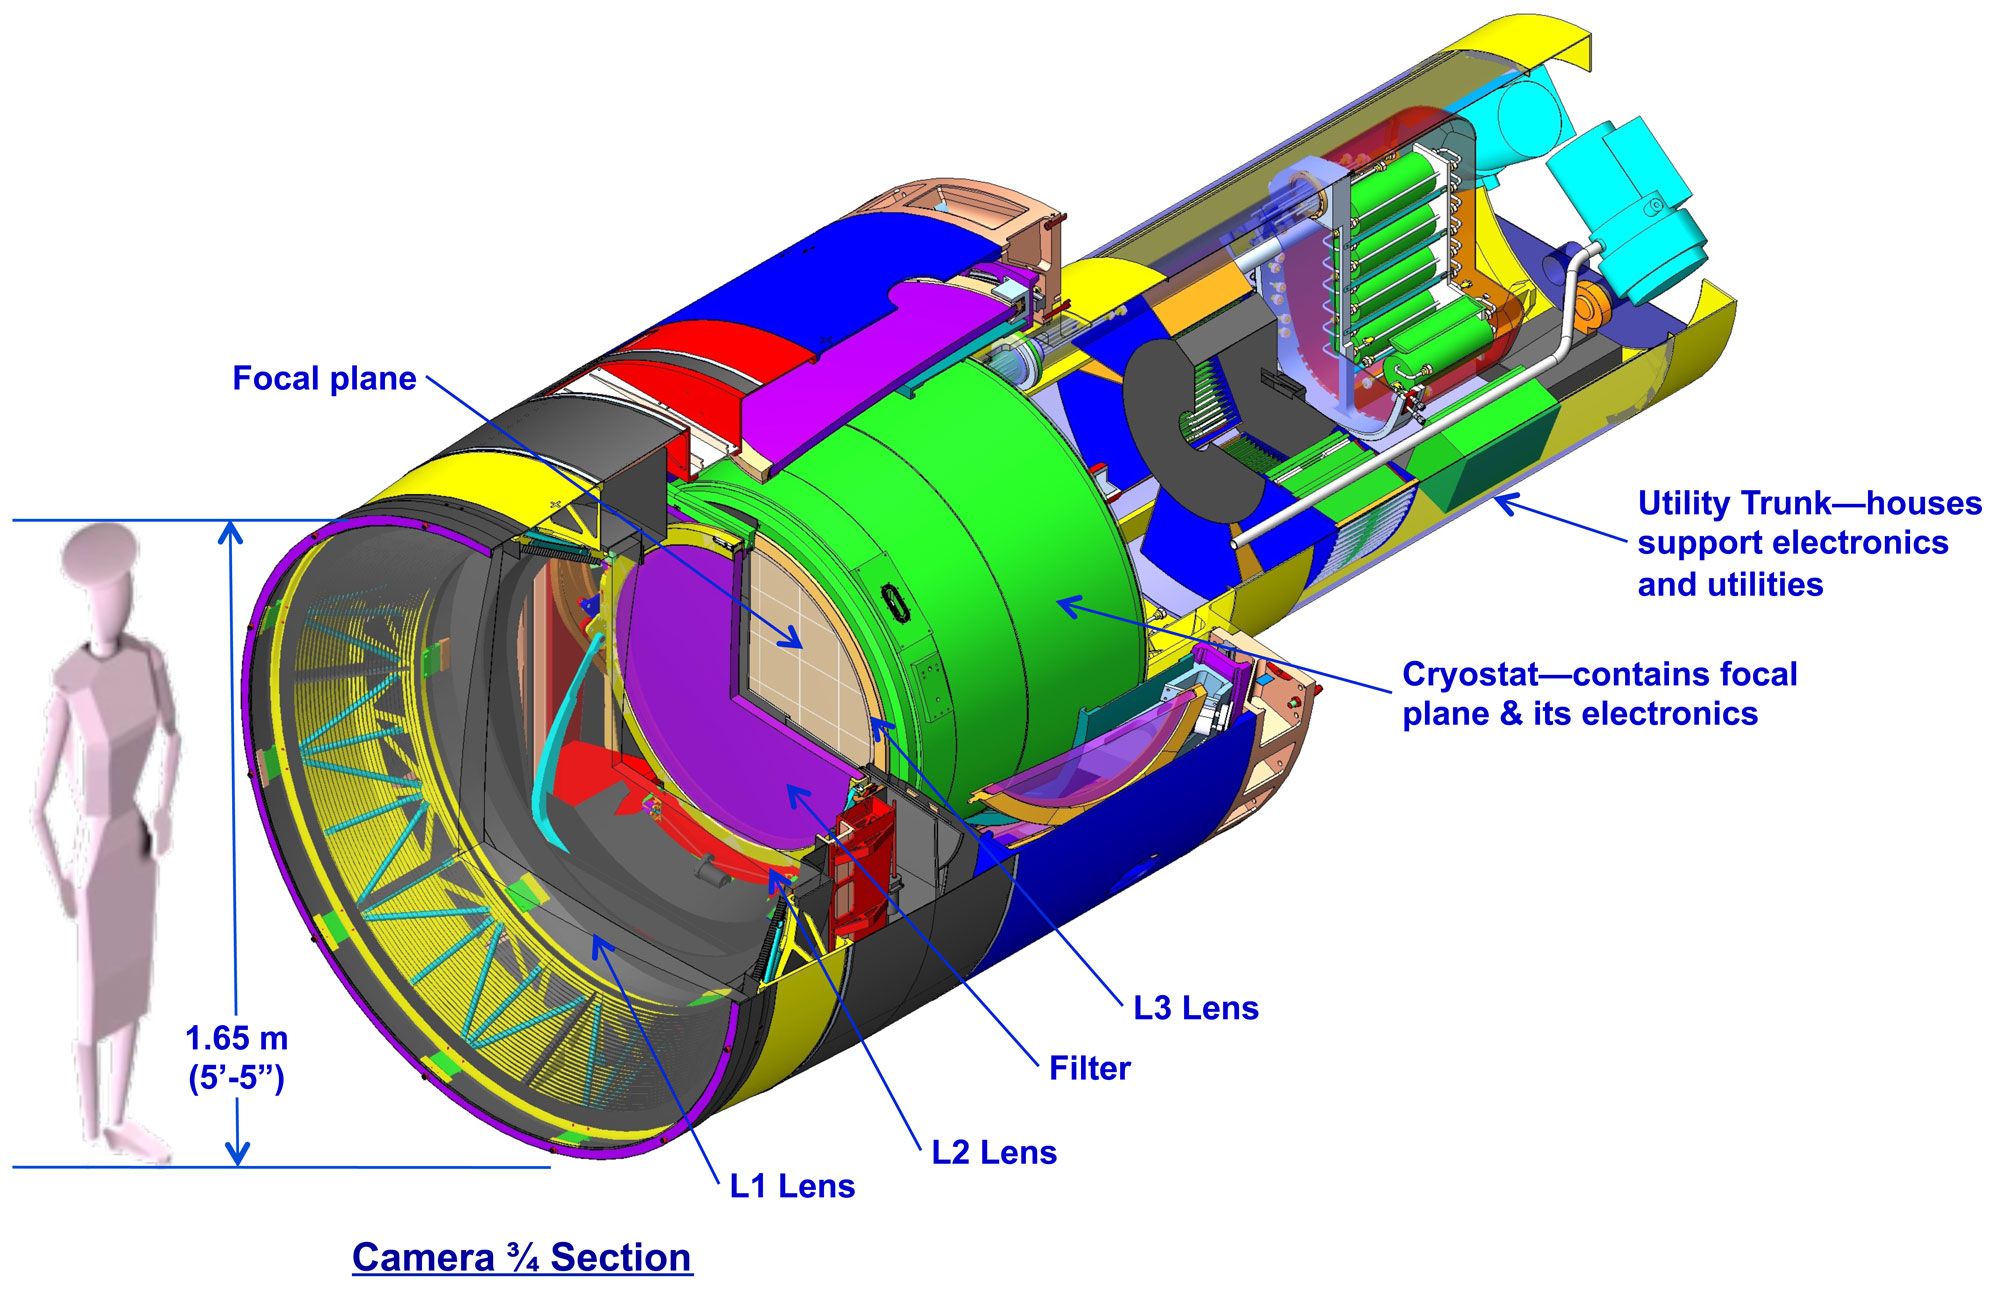
\includegraphics[width=\textwidth]{cosmo_surveys/lsst_cam_design.jpg}
    \caption{A schematic of the LSST camera. The camera body is approximately 1.6 m in diameter and 3.5 m in length. The optic, L1, is 1.57 m in diameter. Credit: SST Project}
    \label{fig:lsst_cam_des}
\end{figure}

Heat dissipation will be be controlled to limit thermal gradients in the optical beam. In order to achieve the desired detector performance, the focal plane array will operates at a temperature of approximately -100\textdegree C. The focal plane array, detector front-end electronics and thermal control are mounted on a silicon carbide grid inside a vacuum cryostat. The cryostat lens serves as an entrance window and vacuum seal for the cryostat. The camera housing is filled with dry nitrogen gas to provide the operating environment for the shutter and filter change mechanisms. The filter carousel can accommodate 5 filters, each 75 cm in diameter, for rapid exchange without external intervention (the sixth filter can replace any of the five via an automated procedure accomplished during daylight hours).

The focal plane consists of 189 arrays ($\sim$16 cm\sq\ each, 3200 cm\sq\ focal plane) of 4k$\times$4k CCDs which should ensure wide field of view while filling the focal plane without any large gaps (less than few hundred \um) -- the fill factor is 93\%. High resistivity silicon substrate and high applied voltages with small pixel size will produce low point spread function (PSF $\ll0.7$ arcseconds). Other focal plane requirements include high quantum efficiency (QE) from 320 to 1080 nm, fast f/1.23 focal ratio, high throughput fast readout (2 sec) or low read noise
\subsection{Auxiliary Telescope}
Along LSST`s construction, a smaller telescope has been assembled on nearby calibration hill, a short distance away from the main LSST Facility. LSST`s 1.2-meter Auxiliary Telescope (AuxTel) will measure atmospheric transmission. Because the presence of certain molecules and particles in the atmosphere will change the color of light detected by the LSST telescope, data collected by the Auxiliary Telescope, as it mirrors the nightly movements of LSST, will inform the catalog corrections that need to be made to LSST data in order to render it more accurate.

AuxTel spectrograph took its first on-sky images on January 27th (see \autoref{fig:AuxTel}). The AuxTel team was able to take data in all modes (both imagery and using dispersers). The images collected represent a significant milestone for system integration and commissioning efforts.

\begin{figure}[ht]
    \centering
    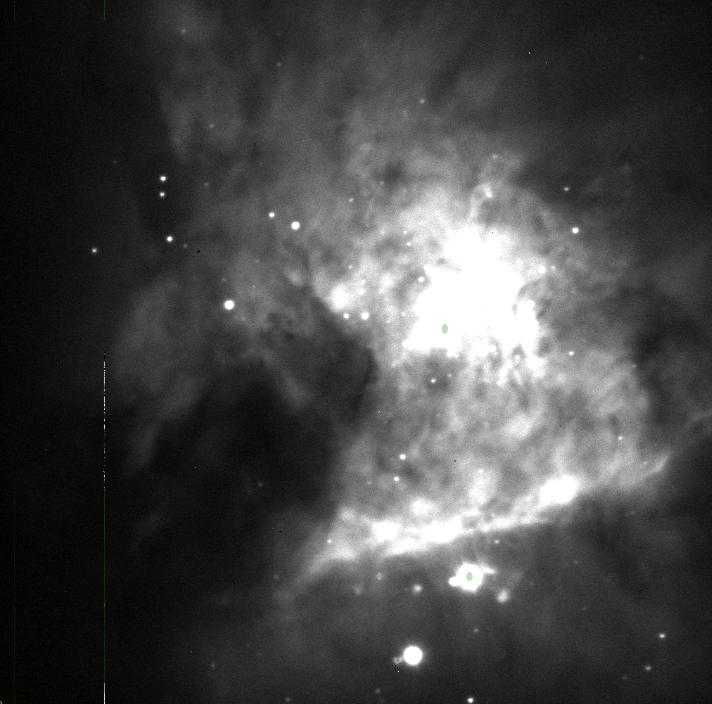
\includegraphics[width=\textwidth]{cosmo_surveys/AuxTelSpec3.png}
    \caption{AuxTel Spectrograph First Light. Credit: LSST Project/NSF/AURA}
    \label{fig:AuxTel}
\end{figure}
\subsection{Data Management}
The LSST Data Management (DM) is responsible for creating the software, services and systems which will be used to produce LSST's data products. DM is required to generate and process a set of data products and to make them available to scientists and the public. DM will create once per year (more often during the first year of the survey) and archives a Data Release (DR), which is a static selfconsistent collection of data products generated from all survey data.

The data management system is architected in three layers: an infrastructure layer consisting of the computing, storage, and networking hardware and system software; a middleware layer, which handles distributed processing, data access, the user interface, and system operations services; and an applications layer, which includes the data pipelines and products and the science data archives. The applications layer is organized around the data products being produced.

\subsection{Dark Energy Science Collaboration}
The LSST Project Team has been assembled to design and build the telescope, camera, and data management systems but it is not a scientific collaboration in the usual sense. While scientists working on the LSST Project are interested in the scientific questions that LSST data can address, they are not officially involved in the scientific analyses of those data. Therefore, a number of quasi-independent scientific collaborations, which provided advices on technical issues and helped articulate the scientific case for the LSST, have created the LSST Dark Energy Science Collaboration (DESC) in 2012 during a meeting at the University of Pennsylvania.

DESC prepares variety of cosmological analyses for the LSST survey. In advance of LSST's first observations, the DESC helps prepare for the LSST science analysis, make synergistic connections with ongoing cosmological surveys and provide the dark energy community with state of the art analysis tools. Primary goal of the DESC is the study of dark energy and related topics in fundamental physics with data from the LSST. For more information see the DESC`s white paper \cite{desc_white}.

Analysis working groups cover five key probes of dark energy: weak lensing, large scale structure, galaxy clusters, Type Ia supernovae, and strong lensing. The DESC will identify and work to minimize the most significant systematic uncertainties that limit the sensitivity of each probe. In addition to these primary goals the DESC will also address joint tasks: calibration strategies for photometric redshifts, cosmological simulations, simulated catalogs, photon-level simulations, cross working group tools, technical coordination (instrument model, calibration and survey operations), and theory and framework for combining and jointly interpreting the dark energy probes.

\section{Planck}
The Planck mission (\cite{planck}) was a European Space Agency mission with significant participation from NASA. It was launched into space on May 14, 2009, and was orbiting the second Lagrange point of our Earth-sun system, about 1.5 million km (930,000 miles) away. Planck was measuring the Cosmic Microwave Background (CMB) over a broad range of far-infrared wavelengths, and to an unprecedented accuracy. Its ultimate goal was to determine the geometry and contents of the Universe, and which theories describing the birth and evolution of the Universe are correct. Planck operated beyond its nominal operational lifetime. It was turned off on 23 October 2013, after nearly 4.5 years soaking up the relic radiation from the Big Bang and studying the evolution of stars and galaxies throughout the Universe's history.

\begin{figure}[ht]
    \centering
    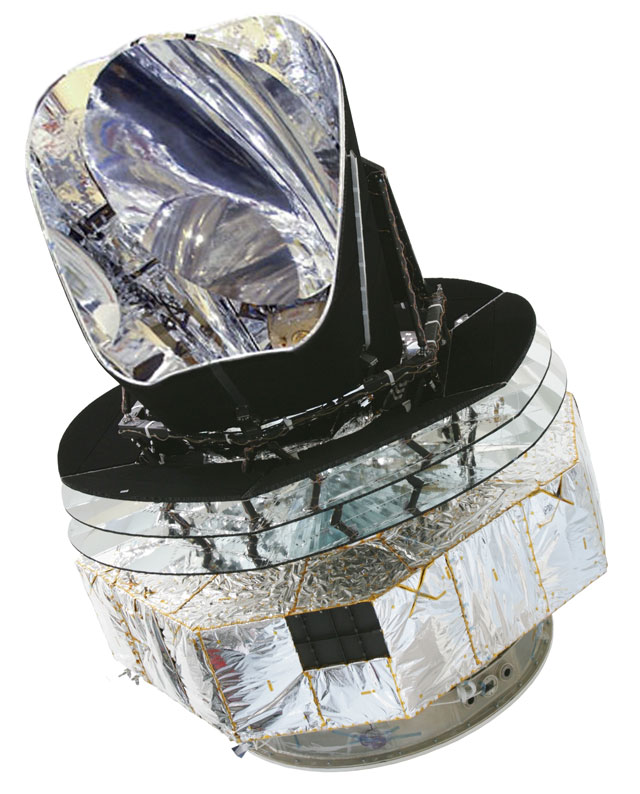
\includegraphics[width=\textwidth]{cosmo_surveys/planck_s.jpg}
    \caption{The Planck satellite.}
    \label{fig:planck}
\end{figure}
The Planck spacecraft was 4.2 metres high and had a maximum diameter of 4.2 metres, with a launch mass of around 1.9 tonnes. The spacecraft comprised a service module, which housed systems for power generation and conditioning, attitude control, data handling and communications, together with the warm parts of the scientific instruments, and a payload module. The payload module consisted of the telescope, the optical bench, with the parts of the instruments that needed to be cooled - the sensitive detector units - and the cooling systems.

The data from Planck have allowed cosmologists to set very tight constraints on many parameters of the standard model, including the Hubble constant, the densities of baryonic matter, dark matter and dark energy, and the spectral index (for Planck results, see \cite{planck_cosm}).

\section{W-FIRST}
The Wide-Field Infrared Survey Telescope (WFIRST) is a NASA large space mission designed to settle essential questions in dark energy, exoplanets, and infrared astrophysics. It is designed to perform wide-field imaging and slitless spectroscopic surveys of the near infrared sky. The current Astrophysics Focused Telescope Assets (AFTA) design of the mission makes use of an existing 2.4-m telescope to enhance sensitivity and imaging performance. It is the top-ranked large space mission in the New Worlds, New Horizon (NWNH) Decadal Survey of Astronomy and Astrophysics. The main instrument is a wide-field multi-filter NIR imager and spectrometer. With the 2.4-m telescope, a coronagraph instrument has been added to the payload for direct imaging of exoplanets and debris disks. If authorized for a mission start in 2017, WFIRST-AFTA would launch in the early 2020s \cite{WFIRST_report}.

\begin{figure}[ht]
    \centering
    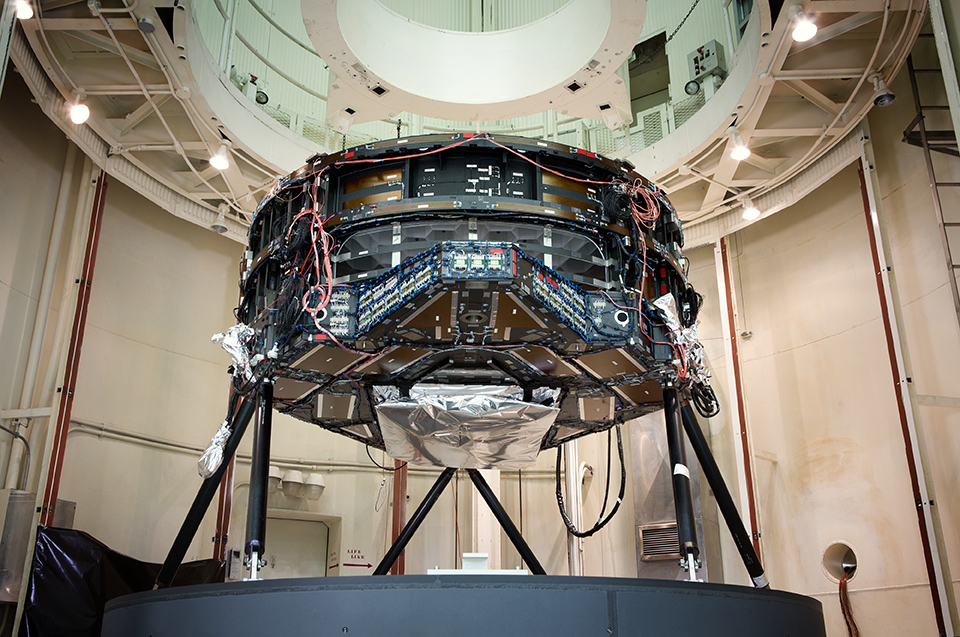
\includegraphics[width=\textwidth]{cosmo_surveys/WFIRST.jpg}
    \caption{Primary Mirror Assembly.}
    \label{fig:wfirst}
\end{figure}
The mission will feature strategic key science programs plus a large program of guest observations. The main focus is on the dark energy and fundamental cosmology (determine the expansion history of the Universe and the growth history of its largest structures). The next scientific goal is discovering of exoplanets -- by microlensing photometric survey of the Galactic bulge and by a direct high-contrast imaging and spectroscopic survey of the nearest stars. Data for general astrophysics science will be gathered by surveys at high Galactic latitudes and Galactic bulge. Relatively huge priority is assigned to the guest observer science program.

The payload features a 2.4-m telescope, which feeds the wide-field instrument (wide-field channel and an integral field unit spectrograph channel) and the coronagraph instrument. The wide-field channel covers a wavelength range 0.76--2.0 \um and a spectroscopy mode covering 1.35--1.89 \um. The wide-field focal plane uses 18 4k $\times$ 4k HgCdTe detector arrays. The integral field unit channel uses an image slicer and spectrograph to provide individual spectra of each slice covering the 0.6--2.0 \um spectral range. The coronagraph instrument provides high-contrast imaging and spectroscopy. Direct imaging is provided over a bandpass of 430--970 nm, while spectroscopy is provided by the spectrograph over the spectral range of 0.6--0.97 \um with a spectral resolution of $R\sim70$ \cite{WFIRST_report}.

As WFIRST will be a NIR mission it will require visible band photometry for photo-z determination. LSST will be the premier ground-based facility to provide those data. As for Euclid, the baryon acoustic oscillation spectroscopic survey will be helpful for calibrating photo-z determinations for LSST. The comparison of shear determinations between WFIRST and LSST measurements will be useful for understanding shape measurement systematics with both facilities.